\documentclass{beamer}
\mode<presentation>
\usepackage{amsmath}
\usepackage{amssymb}
%\usepackage{advdate}
\usepackage{adjustbox}
\usepackage{subcaption}
\usepackage{enumitem}
\usepackage{multicol}
\usepackage{mathtools}

\usepackage{url}
\def\UrlBreaks{\do\/\do-}
\usetheme{Boadilla}
\usecolortheme{lily}
\setbeamertemplate{footline}
{
  \leavevmode%
  \hbox{%
  \begin{beamercolorbox}[wd=\paperwidth,ht=2.25ex,dp=1ex,right]{author in head/foot}%
    \insertframenumber{} / \inserttotalframenumber\hspace*{2ex} 
  \end{beamercolorbox}}%
  \vskip0pt%
}
\setbeamertemplate{navigation symbols}{}

\providecommand{\nCr}[2]{\,^{#1}C_{#2}} % nCr
\providecommand{\nPr}[2]{\,^{#1}P_{#2}} % nPr
\providecommand{\mbf}{\mathbf}
\providecommand{\pr}[1]{\ensuremath{\Pr\left(#1\right)}}
\providecommand{\qfunc}[1]{\ensuremath{Q\left(#1\right)}}
\providecommand{\sbrak}[1]{\ensuremath{{}\left[#1\right]}}
\providecommand{\lsbrak}[1]{\ensuremath{{}\left[#1\right.}}
\providecommand{\rsbrak}[1]{\ensuremath{{}\left.#1\right]}}
\providecommand{\brak}[1]{\ensuremath{\left(#1\right)}}
\providecommand{\lbrak}[1]{\ensuremath{\left(#1\right.}}
\providecommand{\rbrak}[1]{\ensuremath{\left.#1\right)}}
\providecommand{\cbrak}[1]{\ensuremath{\left\{#1\right\}}}
\providecommand{\lcbrak}[1]{\ensuremath{\left\{#1\right.}}
\providecommand{\rcbrak}[1]{\ensuremath{\left.#1\right\}}}
\theoremstyle{remark}
\newtheorem{rem}{Remark}
\newcommand{\sgn}{\mathop{\mathrm{sgn}}}
\providecommand{\abs}[1]{\ensuremath{\left\lvert#1\right\rvert}}
\providecommand{\res}[1]{\Res\displaylimits_{#1}} 
\providecommand{\norm}[1]{\lVert#1\rVert}
\providecommand{\mtx}[1]{\mathbf{#1}}
\providecommand{\mean}[1]{\ensuremath{E\left[ #1 \right]}}
\providecommand{\fourier}{\overset{\mathcal{F}}{ \rightleftharpoons}}
%\providecommand{\hilbert}{\overset{\mathcal{H}}{ \rightleftharpoons}}
\providecommand{\system}{\overset{\mathcal{H}}{ \longleftrightarrow}}
	%\newcommand{\solution}[2]{\textbf{Solution:}{#1}}
%\newcommand{\solution}{\noindent \textbf{Solution: }}
\providecommand{\dec}[2]{\ensuremath{\overset{#1}{\underset{#2}{\gtrless}}}}
\newcommand{\myvec}[1]{\ensuremath{\begin{pmatrix}#1\end{pmatrix}}}
\let\vec\mathbf



\title{Assignment 3}
\author{Teja Vardhan Shannu}
\date{August 2024}

\begin{document}

\begin{frame}
\titlepage
\end{frame}

\begin{frame}
\frametitle{Problem Statement}
A line intersects the Y-axis and the X-axis at the points $ P\brak{0, b} $ and $ Q\brak{c, 0} $ respectively. If $ \brak{2, -5} $ is the midpoint of $ PQ $, find the coordinates of $ P $ and $ Q $.
\end{frame}

\begin{frame}
\frametitle{Problem Data}
\begin{table}[h]
\centering
\begin{tabular}{|c|c|}
\hline
\textbf{Point} & \textbf{Coordinates} \\ \hline
$ P $ & $ \begin{pmatrix} 0 \\ b \end{pmatrix} $ \\ \hline
$ Q $ & $ \begin{pmatrix} c \\ 0 \end{pmatrix} $ \\ \hline
$ M $ & $ \begin{pmatrix} 2 \\ -5 \end{pmatrix} $ \\ \hline
\end{tabular}
\end{table}
\end{frame}

\section{Solution}
\begin{frame}
\frametitle{Midpoint Formula}
Let the coordinates of points $ P $ and $ Q $ be:
\begin{equation*}
\mathbf{P} = \begin{pmatrix} 0 \\ b \end{pmatrix}, \quad \mathbf{Q} = \begin{pmatrix} c \\ 0 \end{pmatrix}
\end{equation*}
The midpoint $ M $ is given by:
\begin{equation*}
\mathbf{M} = \begin{pmatrix} 2 \\ -5 \end{pmatrix}
\end{equation*}
The midpoint formula states:
\begin{equation*}
\mathbf{M} = \frac{1}{2} \brak{\mathbf{P} + \mathbf{Q}}
\end{equation*}
\end{frame}

\begin{frame}
\frametitle{Applying the Midpoint Formula}
Substitute $ \mathbf{P} $, $ \mathbf{Q} $, and $ \mathbf{M} $:
\begin{equation*}
\frac{1}{2} \left(\begin{pmatrix} 0 \\ b \end{pmatrix} + \begin{pmatrix} c \\ 0 \end{pmatrix}\right) = \begin{pmatrix} 2 \\ -5 \end{pmatrix}
\end{equation*}
Simplify to get:
\begin{equation*}
\frac{1}{2} \begin{pmatrix} c \\ b \end{pmatrix} = \begin{pmatrix} 2 \\ -5 \end{pmatrix}
\end{equation*}
Multiplying both sides by 2:
\begin{equation*}
\begin{pmatrix} c \\ b \end{pmatrix} = \begin{pmatrix} 4 \\ -10 \end{pmatrix}
\end{equation*}
\end{frame}

\begin{frame}
\frametitle{Final Answer}
Thus, the coordinates of $ P $ and $ Q $ are:
\begin{equation*}
\mathbf{P} = \begin{pmatrix} 0 \\ -10 \end{pmatrix}, \quad \mathbf{Q} = \begin{pmatrix} 4 \\ 0 \end{pmatrix}
\end{equation*}
\end{frame}

\begin{frame}
\frametitle{Graphical Representation}
\begin{figure}[h!]
\centering
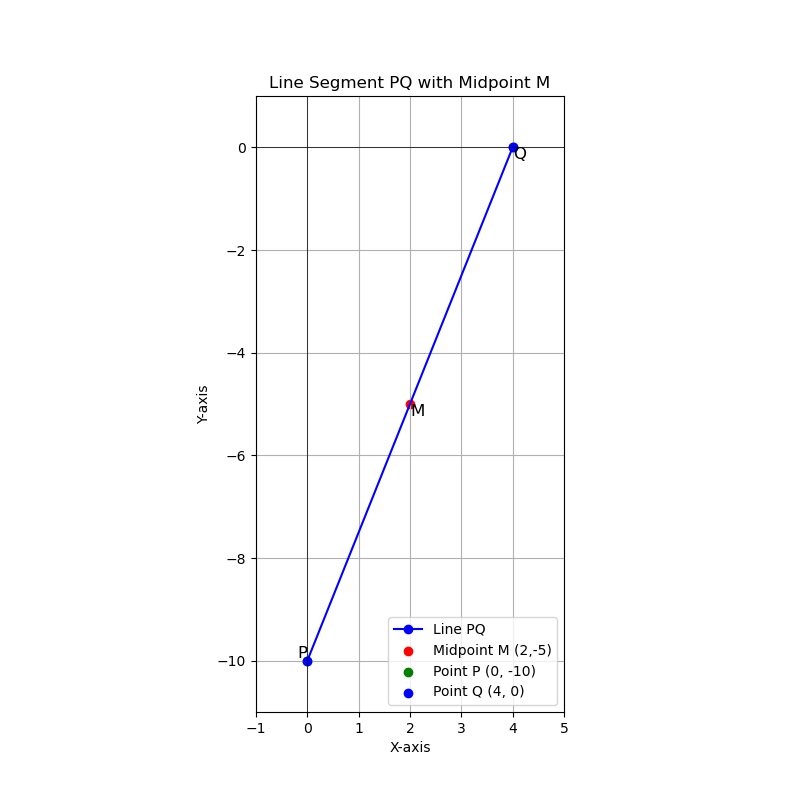
\includegraphics[width=0.7\textwidth]{Figure_1.png}
\caption{Plot showing points $ P $, $ Q $, and midpoint $ M $}
\label{fig:graph}
\end{figure}
\end{frame}

\end{document}


